\section{Validating graphs}\label{sec:valGraph}

\subsection{Graph model}

\subsection{Validation of a graph}

\subsection{Depth-first search}

\subsection{HashSets for depth-first search}

We have finished the last section with a method to check whether a result is a subset of the semantics. For this we need a list of trees representing the result set. Finding such a list is however difficult. Viewing a tree as a set of its elements we see that it is an instance of the NP-hard set cover problem. Additionally, we found in practice that the datalog reasoner we used did only return a list of derivations. Constructing trees from this turned out to be computationally expensive, but the output can be interpreted as a directly acyclic graph. In the following section we describe how to validate such a graph.

A number of different results of graph theory are already proven in mathlib. Nonetheless, we defined our own graph model in Lean for this section due to two main reasons. Firstly, the graph defined in mathlib is a undirected graph, but we require a directed graph so that we can see for a vertex (which represents a ground atom) which neighbors were used to derive it and which neighbors were derived from it. Secondly, the graph represents the edge relation as a map to \texttt{Prop} which is in general not computable.


Our graph model consists of a list of vertices and a function that maps to each element the list of its predecessors. Representing the vertices as a list allows us to iterate over all vertices when validating the graph. We used a function to the predecessors instead of a adjancency matrix similar to the definition in mathlib in order to directly get the predecessors to a node instead of having the iterate over all vertices and check the adjancency matrix. This approach does have a small drawback. Suppose we want to determine whether a property holds for every vertex and do this by exploring the graph using depth-first search and we find a counterexample by following the predecessors. Nothing states that this vertex is actually in the graph, i.e. the list of vertices. This is an undesireable property so that we additionally ask for a proof that the predecessors of every vertex are again vertices in the graph.

\begin{lstlisting}
    structure Graph (A: Type) where
        (vertices: List A)
        (predecessors: A → List A)
        (complete: ∀ (a:A), a ∈ vertices →  
        ∀ (a':A), a' ∈ predecessors a → a' ∈ vertices)
\end{lstlisting}

A standard definition of graph theory are walks as a sequence of connected edges. As we do not have edges directly, we represent this as a list of elements with two properties. A list of elements is a walk in a graph, if all elements are a vertices of the graphs and neighboring vertices are connected via the the predecessor relation of the graph. Due to the completeness property of the graph it would also be sufficient to express that the last element of the path is in the graph. 

\begin{lstlisting}
    def isWalk (l: List A) (G: Graph A): Prop :=
    ( ∀ (a:A), a ∈ l → a ∈ G.vertices ) 
    ∧ ∀ (i: ℕ), i > 0 → ∀ (g: i < l.length), 
    l.get (Fin.mk i.pred (pred_lt i l.length g)) ∈ 
        G.predecessors (l.get (Fin.mk i g) )
\end{lstlisting}

We note that we do allow empty paths. This simplifies some proofs and algorithms even if there is no direct equivalent in graph theory. We specifically use lists as we are going to expand walks at the front when exploring the graph.  

\begin{lemma}
    Let $w$ be a walk in a graph $G$ of the form $a::tl$. Then also $b::a::tl$ is a walk in $G$ for every predecessor $b$ of $a$.
\end{lemma}

Using walks we can define cycles. Every cycle is a walk. Additionally we require that it the start and the end of the walk are equal. In order to have a start and end we have to exclude the empty walks. Additionally, we exclude walks of a single element. Allowing them as cycles would mean that there are no acyclic graphs.

\begin{lstlisting}
    def isCycle (l: List A) (G: Graph A): Prop :=
    if h: l.length < 2
    then False
    else
        have l_not_zero: 0 < l.length :=
        by
        cases ll: l.length with
        | zero =>
            rw [ll] at h
            simp at h
        | succ n =>
            simp

        isWalk l G ∧
            l.get (Fin.mk 0 l_not_zero) 
            = l.get (Fin.mk l.length.pred (Nat.pred_lt (Ne.symm (Nat.ne_of_lt l_not_zero))))
\end{lstlisting}

A graph is then acyclic if no list represents a cycle in it.

\begin{lstlisting}
    def isAcyclic (G: Graph A) := ∀ (l: List A), ¬ isCycle l G
\end{lstlisting}

We need to check whether a given graph is acyclic as only those graphs represent valid derivations. A cycle would mean that we used an atom to derivate itself and we could not get a valid proof tree for this element. We are going to use depth-first search to check whether a graph is acyclic. For this we need an alternative characterization of acyclicity.
A first candidate for this would be the membership in a cycle.

\begin{lemma}
    A graph is acyclic iff no vertice is a member in a cycle.
\end{lemma}

Ideally, we want this characterization to be an iff connection between a vertice and its predecessors. Unfortunately the statement does not hold for this characterization.

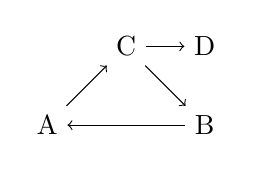
\begin{tikzpicture}
    \node (A) at (0,0) {A};
    \node (B) at (2,0) {B};
    \node (C) at (1,1) {C};
    \node (D) at (2,1) {D};

    \draw[->] (B) -- (A);
    \draw[->] (C) -- (B);
    \draw[->] (A) -- (C);
    \draw[->] (C) -- (D);
\end{tikzpicture}

D is not a member in a cycle, but its predecessor C is, so that an iff does not hold. Instead we see that D can be reached from a cycle using some walk. If it can be reached from a cycle, then also one of its predecessors can be reached from a cycle. We are going to formalize this idea in the following lemmas.

Let $a$ and $b$ be two nodes. We say that $a$ can reach $b$ in $G$ if there exists a walk in $G$ that starts with $a$ and ends with $b$.

\begin{lstlisting}
    def canReach (a b: A) (G: Graph A):= ∃ (w: List A) (neq: w ≠ []),
    isWalk w G ∧
    w.get (Fin.mk 0 (getFirstForNonequal_isLt w neq)) = a ∧
    w.get (Fin.mk w.length.pred (getLastForNonequal_isLt w neq)) = b
\end{lstlisting}

A singleton path allows us to show that any element can reach it self. Additionally, if $a$ can reach $b$ and $b$ is a predecessor of $c$ we can extend the path from $a$ to $b$ with $c$ in order to demonstrate that $a$ can reach $c$. Using the \texttt{canReach} predicate we can now express a different characterization for acyclicity, being reachable from a cycle. A node $a$ is reachable from a cycle $c$, if there exists a node $b$ in the cycle that reaches $a$. In the previous example $D$ is reached from a cycle as $C$ is in a cycle and $C$ reaches $D$. The same holds for $C$ as $C$ reaches itself.

\begin{lstlisting}
    def reachedFromCycle (a:A) (G: Graph A):=
        ∃ (c: List A), isCycle c G ∧ ∃ (b: A), b ∈ c ∧ canReach b a G
\end{lstlisting}

\begin{lemma}
    A graph $G$ is acyclic iff all vertices of $G$ are not reached from a cycle.
\end{lemma}
\begin{proof}
    If $G$ is acyclic, then showing that all vertices of $G$ are not reached from a cycle is equivalent to showing that any cycle in $G$ cannot reach any element. Due to the acyclicity we know that no cycles exist in G so that the first direction is shown.

    The back direction is proved via contradiction. Assuming that the graph is not acyclic, we know that there must exist a cycle $c$ in $G$. Cycles in $G$ are nonempty lists of vertices that are all in $G$. As any vertex can reach itself, there are vertices that are reached from a cycle in contrast to our assumption, so that we have reached the contradiction.
\end{proof}

\begin{lemma}
    A node $a$ is not reached from a cycle iff all predecessors $b$ are not reached from a cycle.
\end{lemma}
\begin{proof}
    Both directions are proven via contradiction. For the first we have that there is a predecessor $b$ of $a$ that is reached from a cycle. Then we can simply extend the path by adding $a$ and then $a$ would be reached from a cycle.

    For the backdirection we assume that $a$ is reached from a cycle and try to show then one of its predecessors must also be reached from a cycle. 
    If $a$ is reached from a cycle $c$ with an element $b$ we consider two cases. 
    If $b$ would be a predecessor, then we have reached a contradiction as $b$ is in the circle and reaches itself. Now we assume that $b$ is not a predecessor of $a$. Again we can consider two cases. If the path is of length one then $a$ and $b$ must be equal and $a$ is a member in a cycle. As long as $a$ is not the first element in the cycle, we can simply pick the preceeding element in the cycle due to the connectness property of the walk. This does not work if $a$ is the first element, but since it is a cycle $a$ must also be the last element and we can pick the predecessor of the last element, which is a predecessor of $a$ and in a cycle.

    If $a$ is reached from a path longer than length 1, we simply pick the subpath without the last element. This is not empty and ends with a predecessor of $a$, which is therefore reached by a cycle. In every case we reached a contradiction so that the claim must be true.
\end{proof}

This completes a characterization of acyclicity that has an iff relation between a node and its predecessors. We still need a method to detect a cycle. We are going to explore the graph via walks and add the current element to the walk whenever we reach a new node. If we see a node again, we have reached a cycle.

\begin{lemma}
    Let $w$ be a walk in a graph $G$ and $a$ be a node of $G$ so that $a::w$ is also a walk in $G$. If $a$ is a member of $w$, then there exists a cycle in $G$.
\end{lemma}

For this we need to extract the walk from $a$ to $a$ out of $a::w$. This is done by the \texttt{getSubListToMember} function. We are given an element $a$, a list $l$ and a proof of $a\in l$ and want to return the sub list until $a$. This is defined inductively. The empty case of $l$ is impossible as $a$ can be a member of the empty list. In the cons case we keep the head element of the list in the result. If this is already $a$, then we stop, else $a$ must be a member in the tail and we continue.

\begin{lstlisting}
    def getSubListToMember (l: List A) (a: A) (mem: a ∈ l): List A :=
    match l with
    | [] =>
        have h: False :=
        by
        simp at mem

        False.elim h
    | hd::tl =>
        if p: a = hd
        then [hd]
        else
        have mem': a ∈ tl :=
        by
            simp[p] at mem
            apply mem
        hd::getSubListToMember tl a mem'
\end{lstlisting}

In any case the list is never empty as we return at least the head of the list we called \texttt{getSubListToMember} on and in both cases the resulting list $l'$ starts with the same element as $l$ used to. By calling it on $w$ with the member $a$ the result $l'$ starts with the same element as $w$. Since $a::w$ was a walk, we therefore can also extend $l'$ with $a$ and preserve a walk assuming that $l'$ preserves a walk. This can be proven by induction. If we have reached the element we return a list with a single element that is a member of $G$, which is always a walk. If not we keep the element and add this to the result of \texttt{getSubListToMember} on the tail. This result is by the induction hypothesis a walk and by the previous result keeps the first element so that we can attach $hd$ again to the front and get a walk. Now we now that the result of \texttt{getSubListToMember a w mem} is a walk and that also \texttt{a::(getSubListToMember a w mem)} is walk. 
In order to show that this a cycle we need two more facts. Firstly, this list should have a length of at least two. This is the case as \texttt{getSubListToMember} never returns an empty list, so that it has at least length one and also attaching $a$ to the front increases the length by one. Secondly, we need the resulting list of \texttt{getSubListToMember a w mem} to end with $a$ so that \texttt{a::(getSubListToMember a w mem)} is cycle. This can again be proven by induction, since the list only ends when $a$ is encountered. 

These facts are enough to start implementing and proving depth-first search in order to check whether the given graph is acyclic. This is however not the only criteria necessary for a valid derivation graph. Additionally, we have to check all steps are valid according to the program as well. We could check this separately, but we will visit all vertices of the graph during the execution of depth first search anyway, so that combining these steps seems more efficient. 

We generalize this by defining depth-first search with a function that takes a vertex and a list of vertices representing the predecessors that is evaluated during the search. We need again a criteria that the depth-first search shall fulfill if it returns acceptance. As we explore the graph want depth-first search to return ok on a vertex $a$ if all vertices reachable from $a$ return ok on the function with their predecessors.

\begin{lemma}
    Let $f:$ \texttt{A → List A → Except String Unit} be a function and $G$ a graph. Then $f$ returns ok for all vertices and their predecessors iff $f$ returns ok for all vertices that can reach a vertex in $G$. 
\end{lemma}
\begin{proof}
    $\Rightarrow$: Any vertex that can reach $a$ in $G$ must also be in $G$. By the assumption therefore $f$ is evaluated to ok on this vertex and its predecessors.

    $\Leftarrow$: As any vertex can reach itself all vertices must return ok when evaluating $f$ with their predecessors.
\end{proof}

Additionally, we see that for every node $a$ all nodes that reach $a$ either reach a predecessor of $a$ or are $a$ themselves.

Now we can define our depth-first search algorithm. In general we follow the definition in \cite{AlgorithmsBook}, but use some helper functions in order to simplify the proofs. Similar to the book we use two main function. A first function \texttt{dfs} calls on all vertices the \texttt{dfs\_step} function that explores graph that can reach this node. In order to not explore a vertex multiple times we return a set of nodes that were already explored. For this we originally used \texttt{Finset} but this turned out to be not fast enough in practice, so that we changed to \texttt{HashSets}.

The function \texttt{addElementIfOk} takes an exception of type \texttt{B} and \texttt{HashSet}. If this exception is ok, i.e. a \texttt{HashSet} it inserts the given element into the hash set. If the exception is an error, we simply return the exception.

\begin{lstlisting}
    def addElementIfOk [Hashable A] (e: Except B (HashSet A)) (a:A):
        Except B (HashSet A) :=
    match e with
    | Except.ok S => Except.ok (S.insert a)
    | Except.error msg => Except.error msg
\end{lstlisting}

From the definition we see that \texttt{addElementIfOk} returns a hash set iff the original exception was already a hash set.

As we are going to call \texttt{dfs\_step} on all predecessors, we use \texttt{foldl} to not explore a vertex multiple times. Our version is a bit modified in order to work with the exceptions. If an error is detected, we stop.

\begin{lstlisting}
    def foldl_except_set [Hashable B] 
    (f: A → HashSet B → (Except String (HashSet B)))
        (l: List A) (init: HashSet B):
        Except String (HashSet B) :=
    match l with
    | [] => Except.ok init
    | hd::tl =>
        match f hd init with
        | Except.error msg => Except.error msg
        | Except.ok S => foldl_except_set f tl S

\end{lstlisting}

The \texttt{dfs\_step} function is called on a vertex $a$ in the graph $G$ together with a function $f$ that shall be evaluated on every vertex and its predecessors in $G$. Additionally, we receive a set \texttt{visited} that contains all explored vertices and the walk \texttt{currWalk} we used in the graph to arrive at the current vertex $a$. In order to prove termination it is important that also \texttt{a::currWalk} is a walk again and that $a$ is not a member of \texttt{currWalk}. As we recursively call \texttt{dfs\_step} we extend the walk by the current node and argue that the number of nodes that are not in the walk decreases. This only works if $a$ is not already present in the walk.

The procedure starts by checking whether the current node is already explored, i.e. \texttt{visited} contains it. If that is the case, we simply return \texttt{visited} and are done. If not we have to explore the graph. Firstly, we check if $f$ is evaluated on the current node and its predecessor to ok. If this is not the case, we have found a counterexample. If it is evaluated to ok, then we check if any predecessor of $a$ is equal to $a$ or in the current walk. This would imply the existance of a cycle and we would report this as an error. 
Finally we call \texttt{dfs\_step} on every predecessor and use \texttt{foldl\_except\_set} to not explore vertices twice. If this returns a hash set, then we add the current node to it. 


\begin{lstlisting}
    def dfs_step [Hashable A] (a: A) (G: Graph A) 
    (f: A → List A → Except String Unit) 
    (currWalk: List A) (walk: isWalk (a::currWalk) G) 
    (not_mem: ¬ (a ∈ currWalk))(visited: HashSet A) :
        Except String (HashSet A) :=
    if visited.contains a
    then Except.ok visited
    else
        match f a (G.predecessors a) with
        | Except.error msg => Except.error msg
        | Except.ok _ =>
        if pred_walk: (G.predecessors a) ∩ (a::currWalk) = []
        then

        addElementIfOk (foldl_except_set (fun ⟨x, _h⟩ S =>
            dfs_step x G f (a::currWalk) 
                (isWalk_extends_predecessors walk x _h) 
                (not_mem_of_empty_intersection pred_walk x _h) S) 
            (G.predecessors a).attach visited
        ) a
        else
            Except.error "Cycle detected"
\end{lstlisting}


The desired property of \texttt{dfs\_step} is the following lemma.

\begin{lemma}\label{lem:dfsstep}
    Let $a$ be a vertex and $S$ be a set such that any member $a'$ of $S$ is not reached from a cycle and that any vertex $b$ that reaches $a'$ is evaluated to \texttt{ok} on $f$. Then \texttt{dfs\_step a G f walk currWalk walk not\_mem S} is evaluated to \texttt{ok} iff $a$ is not reached from a cycle and all vertices $b$ that reach $a$ are evaluated on $f$ with their predecessors to \texttt{ok}.
\end{lemma}

For this we need to determine whether \texttt{foldl\_except\_set} returns an exception or not, which seems dauting due to chaining of results. We get a result for the first predecessors and use this to evaluate the second predecessors and so on and it seemed difficult to determine when its wrong and why. We need this function however to not explore vertices multiple times. This set of previously explored nodes is semantically not so important. We could also work always with the empty set and get the same result with more effort. It only becomes problematic if the set contains elements that are reached from a cycle or an element for which $f$ is not evaluated to ok. We generalize this by considering a property $p$ of vertices and call a function $g$ independent from $p$, if for any node $a$ and sets $S, S'$ whose member both all satisfy $p$, $g( a, S)$ is ok iff $g( a S')$ is ok. This is pretty close to allowing us to consider it as separate calls instead of chaining the results. Additionally we need that $g$ also preserves $p$, i.e. when $S$ is a set whose members all satisfy $p$, then all members of the result $S' = g(a,S)$ also satisfy $p$. Then the initial set can be used instead of the result as both sets only have members that satisfy $p$ and are with respect towards the kind of exception equivalent. Therefore we gain the following lemma by induction to determine the kind of exception of \texttt{foldl\_except\_set}.

\begin{lemma}\label{lem:fes_ok}
    Let $g: A \to HashSet B \to Except String (HashSet B)$ be a function that is independent from a property $p: A \to Prop$ and that preserves $p$. Then for any list $l$ and any hash set $init$ whose members all satisfy $p$, \texttt{foldl\_except\_set} $g$ $l$ $init$ is ok iff $g a init$ is ok for all elements $a$ from $l$.
\end{lemma}

The function $g$ shall represent \texttt{dfs\_step} on the predecessors of a vertex $a$ and $p$ be that a vertex is not reached from a cycle and all elements that reach this vertex are evaluated as ok under $f$. From the induction hypothesis of \ref{lem:dfsstep} we will get the independence from $p$ as the statement of the lemma does not depend on the HashSet at all. Seperatedly we need to prove that \texttt{dfs\_step} preserves the above defined property $p$. The previous lemmas combined the value of for our $p$ on a vertex $a$ with the value of $p$ on $a$'s predecessors. Therefore we want to prove that the resulting set of \texttt{foldl\_except\_set} on the predecessors contains all predecessors and all its members satisfy $p$ in order to conclude that the node $a$ we started from satisfies $p$.

For this we will prove that \texttt{dfs\_step} always returns a subset of the input when it returns ok and need the following lemma for \texttt{foldl\_except\_set}, which can be proven by induction
\begin{lemma}
    Let $g: A \to HashSet B \to Except C (HashSet B)$ be a function so that for all $a$ and $S, S'$, if $g(a,S) = ok S'$, then $S \subseteq S'$. Then also for any list $l$ and sets $S, S'$ with \texttt{foldl\_except\_set} $l$ $S S'$ we have that $S \subseteq S'$.
\end{lemma}

Now we can prove the claim for \texttt{dfs\_step}. The induction for \texttt{dfs\_step} will follow the same structure with the unsatisfiable start and will later be omitted.

\begin{lemma}
    If \texttt{dfs\_step a G f walk currWalk walk not\_mem S} returns a set $S'$, then we have $S \subseteq S'$.
\end{lemma}
\begin{proof}
    We prove this by induction on the number of uncovered vertices by the current path. In the induction basis any vertex is already in the path yet \texttt{not\_mem} tells us that $a$ is not a member in the path, which is a contradiction.
    In the step we do a case distinction whether $a$ is already contained in $S$. If that is the case, then $S$ is returned and due to the reflexivity the claim is proven.
    If not we return the result of a insertion into the result of \texttt{foldl\_except\_set} so that it is sufficient to show that \texttt{foldl\_except\_set} returns a superset of $S$. This is done by the previous lemma together with the induction hypothesis as the path is longer so a smaller amount of vertices is not covered by the path.
\end{proof}

We know that \texttt{dfs\_step} returns a superset of the input set, but what elements are added to this set ? That are essentially all nodes that can reach the node we started our search step from assuming that the visited set already fulfills this property. This theorem is more complicated and for our goals it suffices to know that the starting node is added to the result set assuming it is returned.

\begin{lemma}
    If \texttt{dfs\_step a G f walk currWalk walk not\_mem S} returns a set $S'$ then $S'$ contains $a$.
\end{lemma}
\begin{proof}
    This is proven by case distinction. If $a$ is already contained in $S$, then $S$ is returned and by that the claim is proven.

    If $a$ is not contained in $S$, then the resulting set $S'$ is obtained by inserting $a$ into the resulting set of \texttt{foldl\_except\_set}, so that due to properties of insert $a$ is a member of $S'$.
\end{proof}


Using these two results we have a criteria to show when \texttt{foldl\_except\_set} contains the original list. Due to Lean internal features, the result must be a bit more technical. As we need to show termination in order to unfold our function, we call \texttt{foldl\_except\_set} not on the predecessors of $a$, but instead of the attached version of this list, which is a different type. Therefore we use a function mapping the list type to the set type and refer to the result of this function as the mapped form.

\begin{lemma}
    Let \texttt{f: A → HashSet B → (Except String (HashSet B))} and {g: A → B} be functions such if $f(a,S) $ returns a hash set $S'$  then $S \subseteq S'$ and $g(a) \in S'$. Then for any list $l$ and hash set S,  if \texttt{foldl\_except\_set f l S} returns a hash set $S'$, then for all elements $a$ of $l$, $g(a) \in l$.
\end{lemma}
\begin{proof}
    We prove this by induction on $l$.
    If $l$ is empty all elements of $l$ are in their mapped form in the resulting set.

    If $l$ has the shape $hd::tl$, then we first compute $f(hd,S)$ which must return a set $S'$ since the whole function returns a set. $S'$ must contain $g(hd)$ and is passed into \texttt{foldl\_except\_set} which by the induction hypothesis contains all elements of $tl$ in their mapped form. Due to the subset property all elements of $S'$ must also be contained, so that also $g(hd)$ is in the result. Therefore all elements of the list are contained in their mapped form in the resulting set, if it exists.
\end{proof}

This allows us to show that \texttt{dfs\_step} preserves our property $p$, that is that a vertex $a$ is not reached from a cycle and all vertices that reach $a$ are together with their predecessors evaluated to ok by $f$. For shortness we call this again the property $p$ in the following lemma.

\begin{lemma}
    If \texttt{dfs\_step a G f walk currWalk walk not\_mem S} returns a set $S'$ and all elements in $S$ have the property $p$, then also all elements in $S'$ have the property $p$.
\end{lemma}
\begin{proof}
    This is again proven by the number of vertices not covered by the current walk. 

    In the step we must consider again two cases. If $a$ is already a member of $S$, then $S$ is returned and all elements of $S$ fulfill the property $p$ by assumption. If not then $f(a, G.predecessors(a))$ must be ok. Additionally, \texttt{foldl\_except\_set} must return a hash set $S'$ calling \texttt{dfs\_step} on the predecessors of $a$, which all don't occur in currWalk. Therefore the number of uncovered nodes is smaller, we from the induction hypothesis we know that all these function preserve $p$ and by a separate induction argument also \texttt{foldl\_except\_set} preserves then $p$. The returned hash set is then \texttt{S'.insert a}. As all elements of $S'$ satisfy $p$, we must show that also $a$ satisfies $p$. We know that all predecessors of $a$ are in $S'$.  Firstly, we see that all predecessors of $a$ are in $S'$ and therefore not reached from a cycle, so that also $a$ is not reached from a cycle. Secondly, all elements that reach a predecessor of $a$ fulfill $f$ with their predecessors and also $a$ fulfills $f$ with its predecessors so that $a$ also satisfies $p$.
\end{proof}

Now we have the required tools to finally prove the main lemma \ref{lem:dfsstep} if \texttt{dfs\_step} and do this again by induction.

In the induction step we show both direction seperatedly. First we assume that \texttt{dfs\_step a G f walk currWalk walk not\_mem S} returns a set $S'$. We know that $S$ already had the property $p$ and therefore also $S'$ has the property $p$, which is directly the other direction. Therefore it is enough to show that $a$ is contained in $S'$, which we have already shown.

For the other direction we know that $a$ is not reached from a cycle and all elements that reach $a$ satisfy $f$ and want to show that \texttt{dfs\_step} returns ok. If $a$ is in $S$, then this is the case, so we consider the case of $a$ not contained in $S$. As $a$ can reach itself, $f(a, G.predecessors(a))$ must be ok. Also none of the predecessors of $a$ can occur in the current walk as the would imply a cycle that can reach $a$ in contrast to our assumption. The result is now the result of \texttt{addElementIfOk} which is ok iff the original exception was ok. The original exception is the result of \texttt{foldl\_except\_set}. For this we apply \ref{lem:fes_ok}. The preservation of $p$ was proven before and from the induction hypothesis we see that \texttt{dfs\_step} is independent from $p$, as it being ok does not depend on the set. Additionally, we have to show that all predecessors of $a$ are evaluated to ok on \texttt{dfs\_step}. Using the induction hypothesis this is equivalent to showing that all predecessors are not reached from a cycle and all elements that reach them are evaluated to ok which follows from the assumption. This ends the proof as we have shown both directions.

We have shown the correctness of \texttt{dfs\_step} where we explore all vertices that can reach the start vertices. In order to fully explore the graph, we call this function on every vertex. By using \texttt{foldl\_except\_set} we keep track of the visited vertices, so that we simply return when we already encountered a vertex. 

At the end we do not care anymore about the resulting set and only whether it was ok or if not the error message for which we use the following function for easier proofs. This functions returns ok iff the original returned some element with ok.

\begin{lstlisting}
    def isOkOrMessage (e: Except String A): Except String Unit :=
    match e with
    | Except.error msg => Except.error msg
    | Except.ok _ => Except.ok ()

    def dfs [Hashable A] (G: Graph A) 
    (f: A → List A → Except String Unit) :
        Except String Unit :=

    isOkOrMessage (foldl_except_set 
        (fun ⟨x,_h⟩ S => dfs_step x G f [] (isWalkSingleton G x _h) 
        (List.not_mem_nil x) S)
        G.vertices.attach HashSet.empty 
    )
\end{lstlisting}

This shall return ok iff the graph is acyclic and all its vertices are evaluated to ok with respect to the input function and their predecessors.

\begin{lemma}
    \texttt{dfs G f} returns ok iff $G$ is acyclic and for all vertices $a$ of $G$, $f(a, G.predecessors(a))$ is evaluated to ok.
\end{lemma}
\begin{proof}
    Due to the property of \texttt{isOkOrMessage}, we can replace the left side simply by the \texttt{foldl\_except\_set} on \texttt{dfs\_step}. We know that \texttt{foldl\_except\_set} is ok iff calling \texttt{dfs\_step} on every node with the empty set, which fulfills $p$, returns ok. The prerequisites are fulfilled, because we have proven that \texttt{dfs\_step} preserves $p$ and is independent from $p$ by the semantics lemma. Therefore this is ok, if all vertices of the graph are not reached from a cycle and any vertex reaching a vertex evaluates $f$ to ok with their predecessors. This is equivalent to being acyclic and evaluating $f$ returns ok for any vertex and its predecessors.
\end{proof}

We have designed the depth-first search algorithm to evaluate a function during the search. This function shall inform us that the graph encodes a datalog derivation. This function shall check only a vertex and its predecessors encode a valid datalog derivation, so that we call the property locally valid. This is very similar to the definition of \texttt{isValid} for trees except for the missing \texttt{List.All₂}.

\begin{lstlisting}
    def locallyValid (P: program τ) (d: database τ) (v: groundAtom τ) 
    (G: Graph (groundAtom τ)): Prop :=
    (∃(r: rule τ) (g:grounding τ), r ∈ P 
    ∧ ruleGrounding r g = groundRuleFromAtoms v (G.predecessors v) ) 
    ∨ ((G.predecessors v) = [] ∧ d.contains v)
\end{lstlisting}

The function checking this criteria is again very similar to the one we defined earlier for trees and by a similar argument we show that it is a checker for being locally valid.

\begin{lstlisting}
    def locallyValidityChecker (m: List τ.relationSymbols → List (rule τ))
    (d: database τ) (l: List (groundAtom τ))
    (a: groundAtom τ): Except String Unit :=
    if l.isEmpty
    then
        if d.contains a
        then Except.ok ()
        else checkRuleMatch m (groundRule.mk a l) 
    else
        checkRuleMatch m (groundRule.mk a l)
\end{lstlisting}

\begin{lemma}
    Let $d$ be a database and $a$ a ground atom, that is a vertex in a graph $G$.
    If we use as $m$ the result of \texttt{parseProgramToSymbolSequenceMap} for a program $P$, then \texttt{locallyValidityChecker m d (G.predecessors a) a} returns \texttt{ok} iff $a$ is locally valid in $G$ for $d$ and $P$.
\end{lemma}

Next, we need to use an acyclic graph where all vertices are locally valid to obtain virtual proof trees to show that the vertices are part of the proof-theoretic semantics of datalog. This is done by a function that is similar to depth-first search so that we could reuse its termination argument. The acyclicity of the graph offers us though a different termination argument that simplifies some proofs later.

We already introduced the \texttt{canReach} predicate. All vertices that can reach a vertex $a$ are in some sense a predecessor of $a$. We call all these elements the \textit{global predecessors of $a$}. As any graph is finite and any element that can reach an element in a graph must also be in the same graph, the global predecessors form a finite set. We would like to use the \texttt{Finset.filter} function to gain the predecessors from the finite set of the vertices of a graph. Unfortunately, \texttt{canReach} is not decidable itself (though we can use depth-first search to decide it), which is required to use \texttt{Finset.filter}. Therefore we define an own version of \texttt{Finset.filter} that accepts also by using the original \texttt{Finset.filter} function with the result that any predicate is classically decidable.

\begin{lstlisting}
    noncomputable def Finset.filter_nc (p: A → Prop) (S: Finset A):= 
    @Finset.filter A p (Classical.decPred p) S
\end{lstlisting}

Using classical logic we can also reproof a membership lemma for \texttt{Finset.filter} from mathlib.

\begin{lemma}
    Let $S$ be a finite set and $p$ a predicate and $S'$ be the result of \texttt{Finset.filter\_nc p S}. Then any element is a member in $S'$ iff it is a member of $S$ and $p$.
\end{lemma}

Using this filter allows us to define the global predecessor formally.

\begin{lstlisting}
    noncomputable def globalPredecessors (b:A)(G: Graph A):Finset A:=
    Finset.filter_nc (fun a => canReach a b G) G.vertices.toFinset
\end{lstlisting}

In order to show termination we will need that the global predecessors of a predecessor of $a$ is a strict subset of the predecessors of $a$. Therefore the cardinality of the set of the global predecessors decreases and the algorithm will terminate.

\begin{lemma}
    Let $a$ be a vertex in a graph $G$ and $b$ a predecessor of $a$. Then \texttt{globalPredecessors b G} $\subseteq$ \texttt{globalPredecessors a G}
\end{lemma}
\begin{proof}
    Any element $c$ in \texttt{globalPredecessors b G} has a walk $w$ that ends with $b$. Since $b$ is a predecessor of $a$, $w++[a]$ is also a walk and therefore $c$ also reaches $a$ and is therefore in the global predecessors of $a$. 
\end{proof}

\begin{lemma}
    Let $a$ be a vertex in an acyclic graph $G$ and $b$ a predecessor of $a$.
    Then $a$ is not in the global predecessors of $b$.
\end{lemma}
\begin{proof}
    Suppose that $a$ would be in the global predecessors of $b$. Then we would have a walk $w$ from $a$ to $b$ that has a length of at least one. Then we can again obtain the walk $w++[a]$ that has at least length two and starts and ends with $a$. This would be a cycle in $G$ in contrast to our assumption that $G$ is acyclic. Therefore $a$ can not be a member of the global predecessors of $b$.
\end{proof}

These results suffice the show the termination for the next function. We form a tree by simply taking the current vertex as the root and use the result of all predecessors for the sub trees.

\begin{lstlisting}
    def extractTree (a:A) (G: Graph A) 
    (mem: a ∈ G.vertices) (acyclic: isAcyclic G): tree A :=

    tree.node a (List.map 
    (fun ⟨x, _h⟩ => extractTree x G (G.complete a mem x _h) acyclic) 
    (G.predecessors a).attach)
\end{lstlisting}

The root of the tree that results from \texttt{extractTree a G mem acyclic} is obviously $a$. If we extract for a ground atom $a$ in a graph where any vertex is locally valid, we gain a valid proof tree.

\begin{lemma}
    Let $G$ be a graph of ground atoms, $P$ a program, $d$ a database and $a$ member of $G$. If all vertices of $G$ are locally valid and $G$ is acyclic, then $a$ has a valid proof tree for $P$ and $d$.
\end{lemma}
\begin{proof}
    We proof this by strong induction on the cardinality of the global predecessors for arbitrary $a$. As $a$ is a vertex in $G$ it is locally valid. There are two cases for this.

    We first consider the rule case, i.e. $a$ and its predecessors are an instance of a ground rule from $ground(P)$. We can reuse this rule as the roots of the subtrees are the same as the predecessors of $a$ by our previous assumption. Additionally, all direct subtrees are valid as well by our induction hypothesis. Due to the acyclicity of the graph, the global predecessors of any predecessor $b$ of $a$ form a strict subset of the global predecessors of $a$, so that their cardinality is lower.

    The other option would be that $a$ has no predecessors and is in the database. Then \texttt{extractTree} will add no subtrees, so that the resulting tree is again valid.
\end{proof}

The previous lemma tells us that any vertex in a graph that is acyclic and has only locally valid vertices has a valid proof tree. Therefore the vertices of this graph form a subset of the proof-theoretic semantics and we use the graph validation as an alternative for the tree validation.